\documentclass[a4paper]{article}

\usepackage[english]{babel}
\usepackage[utf8]{inputenc}
\usepackage{amsmath}
\usepackage{amssymb}
\usepackage{graphicx}
\usepackage{bm}
\usepackage[framed,numbered,autolinebreaks,useliterate]{mcode}

\title{SF2955 Project 1 Report}

\author{}

\date{\today}

\begin{document}
\maketitle



\section*{Introduction}

In this project, we use sequential monte carlo methods to estimate the location of a moving object based on cell tower readings.

\section*{Motion model}

% General Information about the motion model
\begin{equation}
\boldsymbol{X}_{n + 1} = \boldsymbol{\Phi X}_n + \boldsymbol{\Psi_Z Z}_n + \boldsymbol{\Psi_W W}_{n + 1}, n \in \mathbb{N} \label{trans_model}
\end{equation}
, where for each n, $\boldsymbol{X}_n = (X_n^1, \dot{X_n^1}, \ddot{X_n^1}, X_n^2, \dot{X_n^2}, \ddot{X_n^2})^T$ \\\\
$\boldsymbol{P}$ is the transition matrix given depicting the transition probability matrix.  
\\\\

% Problem 1 starts here
\textbf{Problem 1}
Is ${\boldsymbol{X_n}}$ a Markov Chain ?  For all $n \in N$, let $\tilde{\boldsymbol{X}_n} = (\boldsymbol{X}_n^T, \boldsymbol{Z}_n^T)^T$, is $\tilde{\boldsymbol{X}_n}$ a Markov Chain ?  Does it look like a reasonable trajectory of a moving target ?\\

%\begin{figure}[ht!]
%\centering
%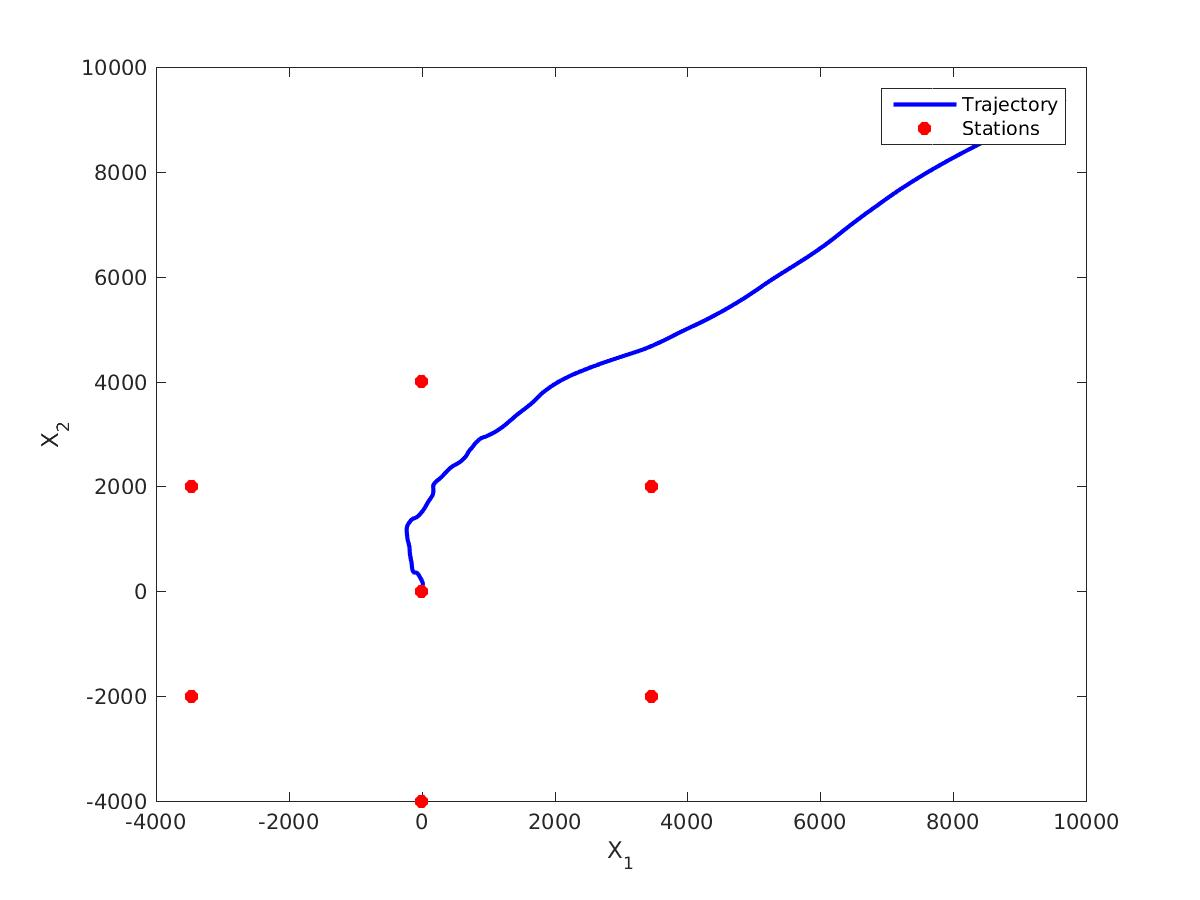
\includegraphics[width=90mm]{q1.jpg}
%\caption{Trajectory generated using the motion model.) \label{q1}}
%\end{figure}

\textbf{Answer:} \\
Yes ${\boldsymbol{X_n}}$ is Markov Chain since it only depends on its previous state ${\boldsymbol{X}_{n-1}}$. \\
Yes, $\tilde{\boldsymbol{X}_n}$ is Markov chain. It also only depends on its previous state. Similar to  ${\boldsymbol{X_n}}$, ${\boldsymbol{Z_n}}$ depicting the driving command just depends on its previous state. Its transition is shown by $\boldsymbol{P}$ matrix. \\

The trajectory in \ref{q1} look like a reasonable trajectory since the direction changes very seldom, because according the transition matrix of driving command state $\boldsymbol{P}$, the probability on staying in the same state is $0.8$ as compared to moving to a different state, which  is $0.2$. Therefore , trajectory is mostly straight with few rare turns.\\

\begin{lstlisting}
global_var; % File Contains all the constants; 

x0 = mvnrnd(mu_x0, sigma_x0); %initialize trajectory
traj(:, 1) = x0'; 
z_index = randi(5,1); %initialize z, selected from uniform dist.

for m = 2:num_steps    
    p = P(z_index, :); %multinomial distribution
    z_index = find(mnrnd(1 ,p ,1));  % sampling from multinomial dist
    z = z_dist(:, z_index); 
    w_n = mvnrnd(mu_w, sigma_w, 1)'; % sampling from motion model 
    x_new = phi*traj(:, m-1) + si_z*z + si_w*w_n; % new state
    traj = [traj x_new];
end

x1 = traj(1,:);
x2 = traj(4,:);

\end{lstlisting}

\section*{Observation model}

%\begin{eqnarray}
%Y_n^l = v - 10\etalog10
%\end{eqnarray}

\textbf{Problem 2}\\
Convince yourself that $\boldsymbol{\tilde{X}_n, \boldsymbol{Y}_n}$ forms a HMM. Find the observation density $p(y_n|\tilde{x}_n)$. \\
\textbf{Answer:} \\
The model $\boldsymbol{\tilde{X}_n, \boldsymbol{Y}_n}$ follows all the principles of a HMM model. First,  $\tilde{\boldsymbol{X}_n}$ is a Markov Chain with transition density given by  Eq.\ref{trans_model}. Secondly, the observations $\boldsymbol{Y}_n$ are independent and conditional distribution of each $\boldsymbol{Y}_n$ depends on the corresponding $\tilde{X}_n$. 

\section*{Problem 1}




\end{document}